\subsection {Langzeitmessung}                                       % 2.3
    \subsubsection{Spannungsverlauf und Leistung}                       % 2.3 a
        \textbf{Methode}
        \newline
        \par Es wurde eine leicht abgewandelte Version der Schaltung aus Abbildung $~\ref{fig:Schaltkreis}$ benutzt, nämlich mit einem konstanten Widerstand von $1\ k\Omega$ anstatt des variablen Widerstandes.
        \par Gemessen wurde am 5.12.2018 am Forum des KIT - Campus zwischen 11:30 Uhr und 13:30 Uhr, mit leichter Bewölkung und einer Temperatur zwischen $10^{\circ}C$ und $15^{\circ}C$.
        \par Die erzeugte Energie wurde mit folgendem Matlab-Skript ausgerechnet:
        
        \begin{figure}[H]
            \lstinputlisting[style=Matlab, frame=single, firstline=17, lastline=25]{messungen/Aufgabe_2_3/import_data.m}
            \caption{Matlab-Skrip zur Berechnung der Energie}
        \end{figure}
        
        \vspace{4mm}
        %\newline
        \noindent
        \textbf{Ergebnis}
        \newline
        \par Folgende Graphen zeigen den Verlauf der Spannung und der Leistung in abhänigeit der Zeit.
        
        \begin{figure}[H]
            %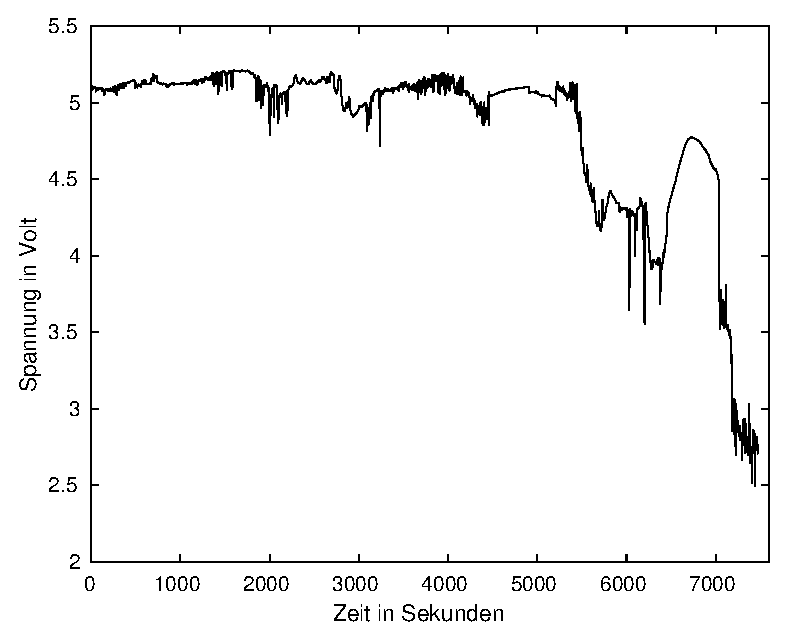
\includegraphics{spannung_langzeit}
            \def\svgwidth{\textwidth}
            \input{spannung_langzeit.pdf_tex}
            
            \caption{Spannungsverlauf über 2 Stunden}
        \end{figure}

        \begin{figure}[H]
            %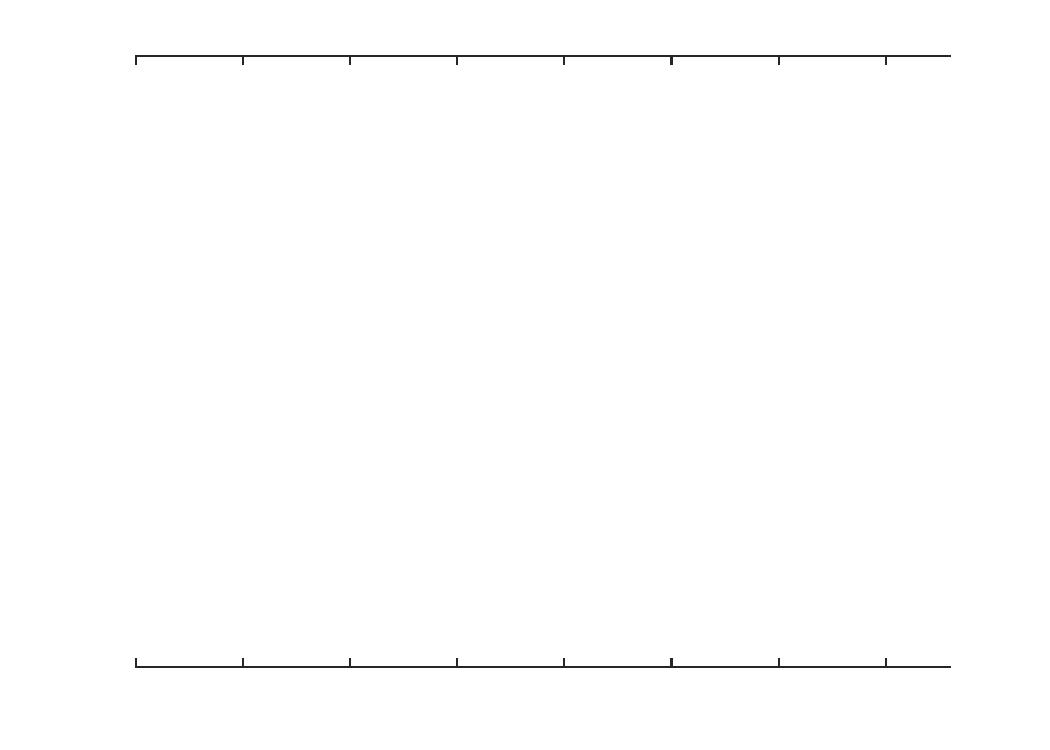
\includegraphics{leistung_langzeit}
            \def\svgwidth{\textwidth}
            \input{leistung_langzeit.pdf_tex}
            
            \caption{Leistungsverlauf über 2 Stunden}
        \end{figure}
        
        Die erzeugte Energie beträgt ungefähr $177.34\ Ws$ bzw. $0.0493\ Wh$.
        \vspace{4mm}
        \newline
        \textbf{Diskussion}
        \newline
        \par Der Energieertrag der Sollarzelle wird bei unterschiedlichen Jahreszeiten durch viele Faktoren wie Temperatur oder der Anzahl der Sonnenstunden beeinflusst, doch der ausschlaggebende Faktor ist der unterschiedliche Winkel, unter dem die Sonnenstrahlung auf die Solarzelle trifft. Ist der Sonnenstand niedriger, wie im Winter, trifft weniger Strahlung auf die Solarzelle und somit wird weniger Energie produziert.
        \par Das Verhältnis sommerlicher und winterlicher Strahlung ist durchschnittlich 3:1 (https://www.solaranlage-ratgeber.de/photovoltaik/photovoltaik-leistung/photovoltaik-ertrag-in-sommer-und-winter, 13.12.2018 21:00 Uhr) und der Energieertrag der Solarzelle hätte im Hochsommer entsprechend bis auf $532.02\ Ws$ bzw. $0.1479\ Wh$ gestiegen.
        
    \subsubsection{Energiegewinnung}                                    % 2.3 b
        \par Die Energiegewinnung mit Solarzellen wird von vielen Faktoren beeinflusst, die von der Umwelt der Solarzelle, aber auch von ader Zelle selbst abhängen.
        \begin{itemize}
            \item Der Winkel in dem die Strahlung auf die Solarzelle eintrifft: Beträgt dieser genau $90^{\circ}$, so ist die Energiegewinnung maximal. Umso größer der Winkel ist, desto kleiner ist die Menge an Strahlung, die von der Solarzelle abgefangen wird.
            \item Die Temperatur: Bei wechselnder Temperatur bleibt die Spannung größtenteils unverändert. Doch je größer die Temperatur ist, desto kleiner wird die Stromstärke die von der Solarzelle ausgeht, und damit auch die Leistung und die Energie.
            \item Das Wetter bzw. Klima: Zum einen beeinflusst es den Einfallswinkel des Lichtes, zum Anderen die Intensität der Strahlung selbst, indem z.B Wolken die direkte Bestrahlung der Zelle verhindern. Die Energiegewinnung mit einer Solarzelle ist also auch Orts- bzw. Zeit-abhänging.
            \item Das Material aus dem die Solarzelle angefertigt wurde: Wird beispielsweise sogennantes monokristallines Silicium verwendet, ist der Wirkungsgrad besonders hoch, ungefähr 25\%. Wird polykristallines Silicium benutzt, fällt der Wirkungsgrad auf 18 - 20 \% und bei amorphem Silicium sind es 5 - 7 \%. 
        \end{itemize}
